\documentclass[a4paper]{article}

\usepackage[english]{babel}
\usepackage[utf8x]{inputenc}
\usepackage[T1]{fontenc}

\usepackage[a4paper,top=3cm,bottom=2cm,left=2cm,right=2cm,marginparwidth=1.75cm]{geometry}

\usepackage{amsfonts}
\usepackage{amsmath}
\usepackage{amssymb}
\usepackage{amsthm}
\usepackage{graphicx}
\usepackage[ruled,vlined]{algorithm2e}
\usepackage[colorinlistoftodos]{todonotes}
\usepackage[colorlinks=true, allcolors=blue]{hyperref}

\setlength\parindent{0pt}

\DeclareMathOperator*{\argmax}{argmax}

\newtheorem{theorem}{Theorem}[section]
\newtheorem{lemma}[theorem]{Lemma}

\title{CS 395T: Homework 1}
\author{Brady Zhou \\ brady.zhou@utexas.edu}

\begin{document}

\maketitle

\section{Linear Algebra}

\textbf{Problem 1.} Derive an expression for $exp(A)$, where

\[
    A = \begin{bmatrix}
            0   & -z    & y \\
            z   & 0     & -x \\
            -y  & x     & 0 \\
        \end{bmatrix}
\]

Let $v \in \mathbb{R}^3$, where

\[
    v = \begin{bmatrix}
            a \\
            b \\
            c \\
        \end{bmatrix}
\]

By expanding $Av$, we can see that

\[
    Av = \begin{bmatrix}
            -zb + yc \\
            za - xc \\
            -ya + xb \\
        \end{bmatrix}
\]

that is, $Av = u \times v$ (cross product matrix), where

\[
    u = \begin{bmatrix}
            x \\
            y \\
            z \\
        \end{bmatrix}
\]

To further understand what $exp(A)$ is doing, we need to pick three linearly independent vectors. \\
For the first vector, choose $\hat u = \frac{u}{||u||}$. \\
For the second vector, pick any $v \in \mathbb{R}^3$ such that $u \perp v$ and $||v|| = 1$ (there is an infinite circle of such vectors). \\
For the third vector, pick $w = \hat u \times v$. This vector is unique given $\hat u, v$, and guaranteed to have unit norm. \\
By choice of these three vectors, we have the following properties.

\begin{itemize}
        \item $A \hat u = 0$
        \item $A v = ||u|| w$
        \item $A w = -||u|| v$
\end{itemize}

First, consider $exp(A) \hat u$.

\begin{align*}
    exp(A) \hat u &= (I + A + \frac{1}{2!} A^2 + \frac{1}{3!} A^3 + \frac{1}{4!} A^4 + \cdots) \hat u \\
                  &= \hat u + 0 + 0 + 0 + \cdots && \text{By } u \times \hat u = 0.
\end{align*}

Next, consider $exp(A) v$, let $\alpha = ||u||$ for simplicity.

\begin{align*}
    exp(A) v &= (I + A + \frac{1}{2!} A^2 + \frac{1}{3!} A^3 + \frac{1}{4!} A^4 + \cdots) v \\
             &= v + \frac{\alpha}{1!} w - \frac{\alpha^2}{2!} v - \frac{\alpha^3}{3!} w + \frac{\alpha^4}{4!} v + \cdots \\
             &= cos(\alpha) v + sin(\alpha) w
\end{align*}

Finally, consider $exp(A) w$.

\begin{align*}
    exp(A) w &= (I + A + \frac{1}{2!} A^2 + \frac{1}{3!} A^3 + \frac{1}{4!} A^4 + \cdots) w \\
             &= w - \frac{\alpha}{1!} v - \frac{\alpha^2}{2!} w + \frac{\alpha^3}{3!} v + \frac{\alpha^4}{4!} w + \cdots \\
             &= -sin(\alpha) v + cos(\alpha) w
\end{align*}

Arranging these into one equations,

\[
    exp(A) \begin{bmatrix}
            \\
            \hat u & v & w \\
            \\
        \end{bmatrix} = \begin{bmatrix}
            \\
            \hat u & v & w \\
            \\
        \end{bmatrix}
        \begin{bmatrix}
            1 & 0 & 0 \\
            0 & cos(\alpha) & -sin(\alpha) \\
            0 & sin(\alpha) & cos(\alpha) \\
        \end{bmatrix}
\]

Which gives the final expression (since $\hat u, v, w$ are ortogonal).

\[
    exp(A) = \begin{bmatrix}
            \\
            \hat u & v & w \\
            \\
        \end{bmatrix}
        \begin{bmatrix}
            1 & 0 & 0 \\
            0 & cos(\alpha) & -sin(\alpha) \\
            0 & sin(\alpha) & cos(\alpha) \\
        \end{bmatrix}
        \begin{bmatrix}
            \\
            \hat u & v & w \\
            \\
        \end{bmatrix}^\intercal
\] \\

\textbf{Problem 2}. Given the following matrix, $A$.

\[
    A = \begin{bmatrix}
        A_{11}            & A_{12} \\
        A_{12}^\intercal  & A_{22} \\
        \end{bmatrix}
\]

If $A \succeq 0$, then $||A|| \leq ||A_{11}|| + ||A_{22}||$.

\begin{proof}
    Let $x$ be the unit eigenvector corresponding with the largest eigenvalue of $A$.

\[
    x = \begin{bmatrix}
        x_1 \\
        x_2
        \end{bmatrix}
\]

Note: since $||x|| = 1$, we have $||x_1||^2 + ||x_2||^2 = 1$. \\

Expanding the term $||A||$,
\begin{align*}
    ||A|| &= x^\intercal A x \\
          &= x_1^\intercal A_{11} x_1 + 2 x_1^\intercal A_{12} x_2 + x_2^\intercal A x_2 \\
          &\leq ||A_{11}||||x_1||^2 + 2 x_1^\intercal A_{12} x_2 + ||A_{22}||||x_2||^2 && (\star)
\end{align*}

Now we must work to get rid of the middle term. Construct a vector $u$
\[
    u = \begin{bmatrix}
        \frac{||x_2||}{||x_1||} x_1 \\
        \frac{-||x_1||}{||x_2||} x_2
        \end{bmatrix}
\]

Since $A \succeq 0$, we have that $u^\intercal A u \geq 0$.
\begin{align*}
    u^\intercal A u &= \frac{||x_2||^2}{||x_1||^2} x_1^\intercal A_{11} x_1 - 2 x_1^\intercal A_{12} x_2 + \frac{||x_1||^2}{||x_2||^2} x_2^\intercal A_{22} x_2 \\
                    &\leq ||x_2||^2 ||A_{11}|| - 2 x_1^\intercal A_{12} x_2 + ||x_1||^2 ||A_{22}|| && (\star \star)
\end{align*}

By construction of $(\star \star)$, adding $(\star \star)$ to $||A||$ cancels out the cross term $2 x_1^\intercal A_{12} x_2$,
\begin{align*}
    ||A|| &\leq (\star) + (\star \star) \\
          &= ||x_1||^2 ||A_{11}|| + ||x_2||^2 ||A_{11}|| + ||x_1||^2 ||A_{22}|| + ||x_2||^2 ||A_{22}|| \\
          &= \big(||x_1||^2 + ||x_2||^2 \big) ||A_{11}|| + \big( ||x_1||^2 + ||x_2||^2 \big) ||A_{22}|| \\
          &= ||A_{11}|| + ||A_{22}|| && \text{By ||x|| = 1}.
\end{align*}

And we have our result.

\end{proof}

\textbf{Problem 3}. Let $A, B \in \mathbb{R}^{m \times n}$. Show $||A \odot B|| \leq ||A|| ||B||$. \\

\begin{proof}

Let $x \in \mathbb{R}^m$, $y \in \mathbb{R}^n$.
\begin{align*}
    ||A \odot B|| &= \argmax_{||x||,||y||=1} x^\intercal (A \odot B) y \\
                  &= \argmax_{||x||,||y||=1} \sum_{i=1}^m x_i \Big((A \odot B) y \Big)_i \\
                  &= \argmax_{||x||,||y||=1} \sum_{i=1}^m x_i \Big( \sum_{j=1}^n (A \odot B)_{ij} y_j \Big) \\
                  &= \argmax_{||x||,||y||=1} \sum_{i=1}^m \sum_{j=1}^n x_i (A \odot B)_{ij} y_j \\
                  &= \argmax_{||x||,||y||=1} \sum_{i=1}^m \sum_{j=1}^n x_i A_{ij} B_{ij} y_j
\end{align*}

To move on, we must use the Cauchy-Shwartz inequality, which states that $(\sum_{i}^{n} a_i b_i)^2 \leq \sum_{i=1}^n a_i^2 \sum_{i=1}^n b_i^2$.
\begin{align*}
    \argmax_{||x||,||y||=1} \sum_{i=1}^m \sum_{j=1}^n x_i A_{ij} B_{ij} y_j
    &\leq \argmax_{||x||,||y||=1}
    \Big( \sum_{i=1}^m \sum_{j=1}^n (A_{ij} x_i)^2 \Big)^\frac{1}{2}
    \Big( \sum_{i=1}^m \sum_{j=1}^n (B_{ij} y_j)^2 \Big)^\frac{1}{2} \\
    &= \argmax_{||x||,||y||=1}
    \Big( \sum_{i=1}^m \sum_{j=1}^n A_{ij}^2 x_i^2 \Big)^\frac{1}{2}
    \Big( \sum_{i=1}^m \sum_{j=1}^n B_{ij}^2 y_j^2 \Big)^\frac{1}{2} \\
    &= \argmax_{||x||,||y||=1}
    \Big( \sum_{i=1}^m x_i^2 \sum_{j=1}^n A_{ij}^2 \Big)^\frac{1}{2}
    \Big( \sum_{i=1}^m \sum_{j=1}^n B_{ij}^2 y_j^2 \Big)^\frac{1}{2} \\
    &= \argmax_{||x||,||y||=1}
    (\star)
    (\star \star)
\end{align*}

Now, let us work on $(\star)$.
\begin{align*}
    (\star) &= \argmax_{||x|| = 1}
    \Big( \sum_{i=1}^m x_i^2 \sum_{j=1}^n A_{ij}^2 \Big)^\frac{1}{2}
\end{align*}

Since $||x|| = 1$, this is a convex combination of the l2-norms of $A$'s rows. Trivially, this is maximized by picking the row with the highest l2-norm.
\begin{align*}
    \Big( \sum_{i=1}^m x_i^2 \sum_{j=1}^n A_{ij}^2 \Big)^\frac{1}{2} &= \argmax_{1 \leq i \leq m} (A^\intercal)_i \\
                                                                     &= \argmax_{x \in \{e_i : 1 \leq i \leq m \}} ||A^\intercal x|| \\
                                                                     &\leq ||A^\intercal|| \\
                                                                     &= ||A||
\end{align*}

Similarly, $(\star \star)$ can be thought of picking the column with the highest l2-norm.
\begin{align*}
    (\star \star) &= \argmax_{||y|| = 1}
    \Big( \sum_{i=1}^m \sum_{j=1}^n B_{ij}^2 y_j^2 \Big)^\frac{1}{2} \\
    &= \argmax_{1 \leq i \leq n} ||B_i|| \\
    &= \argmax_{x \in \{e_i : 1 \leq i \leq n \}} ||B x|| \\
    &\leq ||B||
\end{align*}

In the definition of vector-induced matrix norm, we can pick any vector that belongs in the same column space. We can see the the last step is true since the set of basis vectors we are ``argmaxing'' over is now a subset of the original column space. \\

Combining the two facts, we have that $||A \odot B|| \leq ||A|| ||B||$.
\end{proof}

\section{Probability}

\textbf{Problem 6.} Show that the probability of capturing the origin with tetrahedron formed by picking four random points on the unit sphere is $\frac{1}{8}$. \\

Without loss of generality let the first three points be $A$, $B$, $C$. Clearly these form a triangle. Let $A^\prime$, $B^\prime$, $C^\prime$ be the corresponding projections through the origin to the other side of the sphere.

\begin{figure}[!h]
\centering
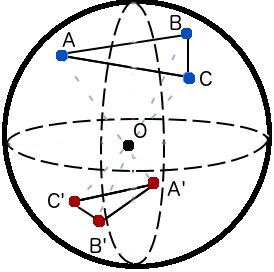
\includegraphics[width=0.2\textwidth]{spherepoints.png}
\caption{Triangle ABC and the projected points through the origin. Graphic crudely and painfully constructed in photoshop.}
\end{figure}

We can see that $A, B, C, A^\prime, B^\prime, C^\prime$ form a triangulation across the sphere that forms a total of 8 regions. These regions are the triangles $A B C, A^\prime B^\prime C^\prime, A B C^\prime, B C A^\prime, C A B^\prime, A^\prime B^\prime C, B^\prime C^\prime A, C^\prime A^\prime A$ projected onto the sphere. \\

Consider which tetrahedra are formed depending on the placement of the last point $D$. If $D$ is placed within the region $A^\prime B^\prime C^\prime$, then the tetrahedron will capture the origin. This can be seen by taking the barycentric coordinates of the origin with respect to the tetrahedron $A B C D$ and verifying that the coordinates are a convex combination of $A, B, C, D$. If the point $D$ lies in any of the other 7 regions, then the origin is not captured. \\

Ignoring degenerate cases such as $D$ falling on the boundary of the region $A^\prime B^\prime C^\prime$, in which the origin would lay exactly on a face of the tetrahedron (we can ignore this since the probability this specific instance is 0), we can see that the 8 regions above cover the same area when picking random points, which gives us our result that the probability of capturing the origin with a tetrahedron formed by picking four random points is $\frac{1}{8}$. \\

\textbf{Problem 7.} Given a set of $n$ numbers $0 \leq i < n$ arranged in a circle, show that the probability $p_i$ of landing on number $i$ starting for $0$ is $\frac{1}{n-1}$, for $i \neq 0$.

\begin{lemma}
    Gambler's ruin (Stated without proof). Let $W$ denote the event of obtaining $n$ coins without losing all coins. Let $P(W | X_0 = k)$ denote the probability of winning a total of $n$ coins, starting with $k$ coins. $P(W | X_0 = k) = \frac{k}{n}$.
\end{lemma}

With the previous lemma, this problem is near trivial. Consider the following scenario of being on spot $0$, and we wish to calculate the probability that when landing on spot $i$, we have landed on all other spots previously. There are two ways of landing on $i$ such that this is achieved. \\

First, consider the probability of landing on $i-1$ from the clockwise direction, without ever landing on $i$ from the counter clockwise direction. This is equivalent to the Gambler's ruin scenario starting with $n-i$ coins, and trying to achieve a goal of $n-1$ coins, so the probability of this scenario is $\frac{n-i}{n-1}$. Now from position $i-1$, there are still positions to be touched. The probability of reaching $i$ from the counter clockwise direction (going all the way around), without ever hitting $i$ from the clockwise direction is equivalent to winning $n$ coins, starting with $1$ coin, which gives a probability of $\frac{1}{n}$. The total probability of this occuring (CW, then CCW), is $\frac{n-i}{n-1}\frac{1}{n}$. \\

Next, we must determine the probability of CCW, then CW. The probability of reaching $i+1$ from the counterclockwise direction, starting from position $0$ is equivalent to winning $n-1$ coins, starting with $i$ coins. From there, the probability of reaching $i$ from the clockwise direction without ever hitting $i$ from the counterclockwise direction is equivalent to winning $n$ coins, starting with $1$ coin. This gives a total probability of $\frac{i}{n-1}\frac{1}{n}$. \\

Adding these two probabilities together, since either one could occur, we have $p_i = \frac{n-i}{n-1}\frac{1}{n} + \frac{i}{n-1}\frac{1}{n}$. With a bit of algebraic manipulation, we have our result - that $p_i = \frac{1}{n-1}$, for $0 < i < n$.

\section{Geometry/Topology}

\textbf{Problem 12}. Show that for a maximally planar graph, we have that a 4-coloring of the vertices implies a 3-coloring of the edges, and that a 3-coloring of the edges implies a 4-coloring of the vertices.

\begin{proof} A 4-coloring of the vertices implies a 3-coloring of the edges. \\

    Let $RGBA$ denote the colors of the vertices. First, we will show a 4-coloring implies a 6-coloring trivially, and then map this 6-coloring into a 3-coloring. For our 6-coloring, we will se the colors by choosing two of the vertex colors in arbitrary order. Clearly there are $4\choose2$ edge colors, $RG, RB, RA, GB, GA, BA$. Consider each edge and it's corresponding $u, v$ vertices. Without loss of generality, for each edge, if $u$ has a color $R$, and $v$ has a color $G$, we will color this edge $RG$. \\

    To show this forms a 6-coloring, on the contrary, if this did not form a 6-coloring, consider the violiating triangle $uvw$. Without loss of generality, $uv$ and $uw$ would both have edge color $RG$. By construction, the only way this could occur is if $u$ had color $R$, and $v, w$ have color $G$. We can see this violates the 4-coloring assumption for the vertices. Contradiction. We can see we have constructed a 6-coloring of the edges. \\

    Next, we need to find a mapping $M$ from our 6-coloring to a 3-coloring of colors $X, Y, Z$. To construct this, let $M$ be the following map - $RG, BA \rightarrow X$; $RB, GA \rightarrow Y$; $RA, GB \rightarrow Z$. We can see that for every mapping, the vertices $RGBA$ are only used a single time. To show this mapping successfully obtains a 3-coloring, consider the contrary. Let $uvw$ be the violating triangle such that two edges $uv$, $uw$ have the same edge color $X$. This ensures $uv$ former color was $RG$ and $uw$ former color was $BA$ (otherwise the original 6-coloring would be violated). If edge $uv$ is colored $RG$, then this implies vertex $u$ is either colored $R$ or $G$, but if edge $uw$'s former color is $BA$, this implies vertex $u$ has a color of either $B$ or $A$. Contradiction. We can see that we have successfully constructed a 3-coloring of the edges.

\end{proof}

\begin{proof} A 3-coloring of the edges implies a 4-coloring of the vertices. \\

    To construct the coloring, we need the map $M$ from the previous proof. The procedure for coloring the vertices is as follows. Pick any arbitrary triangle $uvw$ to start from. From this triangle, pick the edge $uv$, with the corresponding edge color $X$. From the map $M$, we have two options to color the vertices $RG$, or $BA$. Without loss of generality, set $u$ to be $R$, and $v$ to be $G$. Now, to color the vertex $w$, look up the reverse mapping of $uw$'s edge color $Y$. By construction of the map, there will be a pair $RB$, and $GA$, to generalize, $RQ$, and $ST$, where $QST$ are unique and not the color $R$. This means vertex $w$ is the unknown color $Q$ ($B$ in this case). To show this is consistent, look at the edge $vw$, with the corresponding color $Z$. The reverse mapping gives a choice of $GB$, and $RA$. Clearly, we pick $GB$, which is consistent with our previous choice that $w$ is colored $R$ and $v$ is colored $G$. If we continue this greedy color selection, by construction of the map $M$, we are guaranteed to use a maximum of 4 vertex colors that are non-incident and we are done.

\end{proof}

\end{document}
